\chapter{Introduction}

Nearly everything around us has been \textit{designed} and
\textit{built}. With mass production, a single design can be
replicated many times. This keeps prices low and quality consistent,
but users must be content with what the designer and manufacturer have
done.

But what if the user could indicate exactly what they want for the
same price and quality? Machines like 3D printers, CNC mills, and
laser cutters are beginning to give a glimpse of what the future might
hold. Today, a knowledgeable person can design and ``print'' parts on
rapid prototyping machines. If the designer wants to change something,
they simply print a revision. While this is currently not as
cost-effective as buying an ``almost good enough'' mass-produced
product, it does enable the user to directly engage with designing and
making.

Rapid prototyping is a new technological phenomenon with economic and
social consequences. The machinery that enables regular people to
``print'' objects at home was unavailable ten years ago: either it was
too expensive, or it had not yet been invented. 

Current prototyping machinery is still too expensive for most people
to buy for personal use. But this will likely change in the coming
years as more machines become available. The market for rapid
fabrication machines is growing quickly: according to industry
analysts, the market for laser cutters will exceed \$3.8 billion by
2015, and the 3D printer market will reach \$3.1 billion by
2016~\cite{laser-cutter-market,3d-printer-market}.

Today's machines produce adequate (but not typically compelling)
output. This is quickly changing as price decreases while quality
improves. We are witnessing the start of a technology that enables new
activities---some that we can predict, but others that we can not yet
clearly see. It is conceivable that we are witnessing the beginning of
a shift from an economy entirely based on \textit{mass production} to
one that includes \textit{mass customization}.

Rapid fabrication gives many people the ability to design and build
things when there was no opportunity before. In the mass production
model, people are merely consumers. Rapid fabrication enables people
to play an active role in designing and constructing the world around
them. \textit{However, the machines, alone, are insufficient: a human
  must tell them what to make. To support this, people need adequate
  design tools}.

This dissertation addresses the observation that people need better
design tools if they are to effectively use rapid fabrication
machines. Current modeling software targets users who go to school to
learn how to design and use design software. But most people can not
dedicate that much time to learn the intricacies of design software.

\begin{figure}[t]
  \centering
  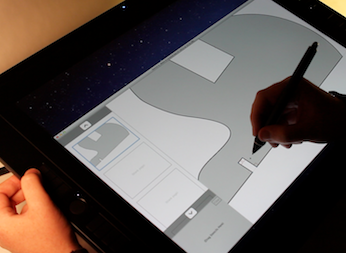
\includegraphics[width=0.9\linewidth]{img/simi-with-cintiq.png}
  \caption[SIMI on a Wacom Cintiq]{Using Sketch It, Make It on a Wacom
    Cintiq display tablet. The user sketches with their preferred
    hand, and uses a single button with their non-dominant hand.}
  \label{fig:simi-intro}
\end{figure}

While someone might find professional design software to be difficult,
it is likely that person can \textit{draw} with pencil and paper to
communicate ideas with others. Even if the sketch is rough, it is an
effective method to express ideas about form and function.

\section{Thesis Statement and Contributions} 

\begin{quote}
\textbf{Thesis Statement}: Sketch-based interaction can provide the
basis for a useful and usable 2D modeling tool for designing laser cut
items.
\end{quote}

Researchers have attempted to leverage sketching as a computational
medium for at least half a century. But we have not seen this effort
move beyond academic laboratories. A critical element missing from
this body of work is the lack of a \textit{system of interaction
  design} for sketch-based tools.

I offer several \textbf{Contributions} to support my thesis. First, I
present a coherent set of sketch-based interaction techniques that
enables users to make precise designs with a stylus. Second, I develop
several new interaction techniques including Flow
Selection~\cite{johnson-flow-selection}. Last, I offer a recognition
and disambiguation architecture that supports fast and user-friendly
interaction design.

These contributions are embodied in a \textit{useful} and
\textit{usable} modeling tool called \textit{Sketch It, Make It
  (SIMI)} that lets people design precise items for laser
cutters.

\section{Intended Audience}

This work is aimed primarily at researchers interested in sketch-based
modeling---particularly those developing sketch recognizers or
interactive sketch-based software systems. This includes people
working on topics traditionally found in computer science
(e.g. artificial intelligence or computer graphics) as well the
human-computer interaction and interaction design communities. Beyond
motivating the work (sketch-based interaction) and domain (designing
for laser cutters), a reader could implement any of the techniques
described herein. The target audience may be in academia, but it is
hoped that commercial software tools can start to incorporate some of
the novel interaction exemplified by SIMI.

Further, members of the physical hacking or tangible interaction
worlds may be interested in learning how their trade can benefit from
improved design tools.

\section{Motivation}

This work is motivated by academic and practical perspectives. From an
academic perspective, I am motivated to find a way to bring greater
coherence to the field of sketch-based modeling with a compelling
example of a useful and usable sketching system that exhibits a set of
mutually harmonious interaction techniques. There are dozens of
sketch-based systems that demonstrate recognition algorithms,
corner-finding methods, and interaction techniques, among other
topics. But as I have said, sketch-based tools don't exist outside
research labs. Because researchers rarely share, or have complete
documentation or working examples to use as a starting point, they
must typically build their work from scratch. Consequently,
researchers interested in one topic (e.g. making new interactive
widgets for sketching) must spend a substantial amount of time
implementing functions that are not their research focus (e.g. ink
parsing). Although it might occasionally be a useful learning strategy
to re-invent the wheel, I view the focus on side-topics as a largely
needless distraction.

The practical motivation behind this work is the observation (shared
by many people) that current computer-based design tools are hard to
use, and that ``natural'' techniques like drawing, speaking, and
gesturing are potentially great methods to design with computers. It
would be a wonderful turn of events if such a natural, easy-to-use
tool were available to designers. I believe one of the critical steps
to making this a reality is to develop an appropriate system of
interaction. For example, such a system to interact with (drive) a car
involves foot pedals, a steering wheel, and dashboard indicators and
knobs. It would be inappropriate (and dangerous) to force automobile
drivers to control their cars with a standard PC setup: keyboard and
mouse, complete with software updates and dialog boxes. But this is
the approach that many researchers take when developing sketch-based
design tools. It is convenient, but inappropriate. This dissertation
offers an example of an appropriate interaction for sketch-based
design tools.

\section{Thesis Structure}

This chapter introduced the domain of rapid fabrication and the
culture of hacking and making that is associated with it.  I discussed
the field of sketch-based modeling and introduced my tool,
\textit{Sketch It, Make It (SIMI)}, a digital modeling tool for
designing precise items for laser cutters. The following chapters are
outlined as follows.

Chapter 2 covers background information about rapid fabrication and
laser cutting, and provides a brief survey of the literature on
computational support for sketch-based modeling in design. Next, in
Chapter 3 I describe formative investigations that informed
development of my tool: observations and interviews with designers,
and an analysis of some of the artifacts made with current design
tools and laser cutters.

Two chapters are devoted to discussing SIMI. Chapter 4 introduces the
tool and presents usage scenarios: why and how somebody uses it. This
is an overview of the system. Chapter 5 details individual interaction
techniques and other technical aspects to the system likely to be
useful to others.

Chapter 6 presents several evaluations of SIMI, including results of a
quantitative evaluation involving 60 undergraduate architecture
students. Last, in Chapter 7, I discuss the implications SIMI has on
digital modeling tools and sketch-based design. I also describe some
additional questions that warrant future work.
